\documentclass{beamer}
\usetheme{Berkeley}
\usecolortheme{seahorse}
\usepackage{hyperref}
\usepackage{graphicx}
\usepackage{amsmath}
\def\bm#1{\mbox{\boldmath $#1$}}
\include{macros}
 
\title{Designs for subsampling tree cores for biomass estimation}
\author{John Tipton, Mevin Hooten }
\date{\today}
\begin{document}
%
\begin{frame}
  \maketitle
\end{frame}
%
\begin{frame}
  \frametitle{Introduction}
  \section{Introduction}
  Goals
  \begin{itemize}
    \item Estimate plot level biomass with increased precision \vspace{3mm}
    \item Increase the number of large dbh trees in the sample \vspace{3mm}
    \item Easily implementable in the field
  \end{itemize}
\end{frame}
%
\begin{frame}
  \frametitle{Biomass Model}
  DBH is used as a predictor for biomass using an allometric equation.   Under simple random sampling, the model of interest is the allometric tree growth equation with exponential error given by 
  \begin{align}
  \label{1}
     y_i & =  x_i^{\beta_1} e^{\beta_0 + \epsilon}
  \end{align}
  where $y_i$ is biomass for tree $i$, $x_i$ is dbh for tree $i$, $\epsilon \sim N(0, \sigma^2)$ is a random error, and $\beta_0$ and $\beta_1$ are coefficients to be estimated.
\end{frame}
%
\begin{frame}
  \frametitle{The Model}
  A plot of the allometric relationship using simulated data
  \begin{figure}
    \centering
%     \caption{Plot of simulated allometric relationship typical of a sample plot (assumes one species only)}
    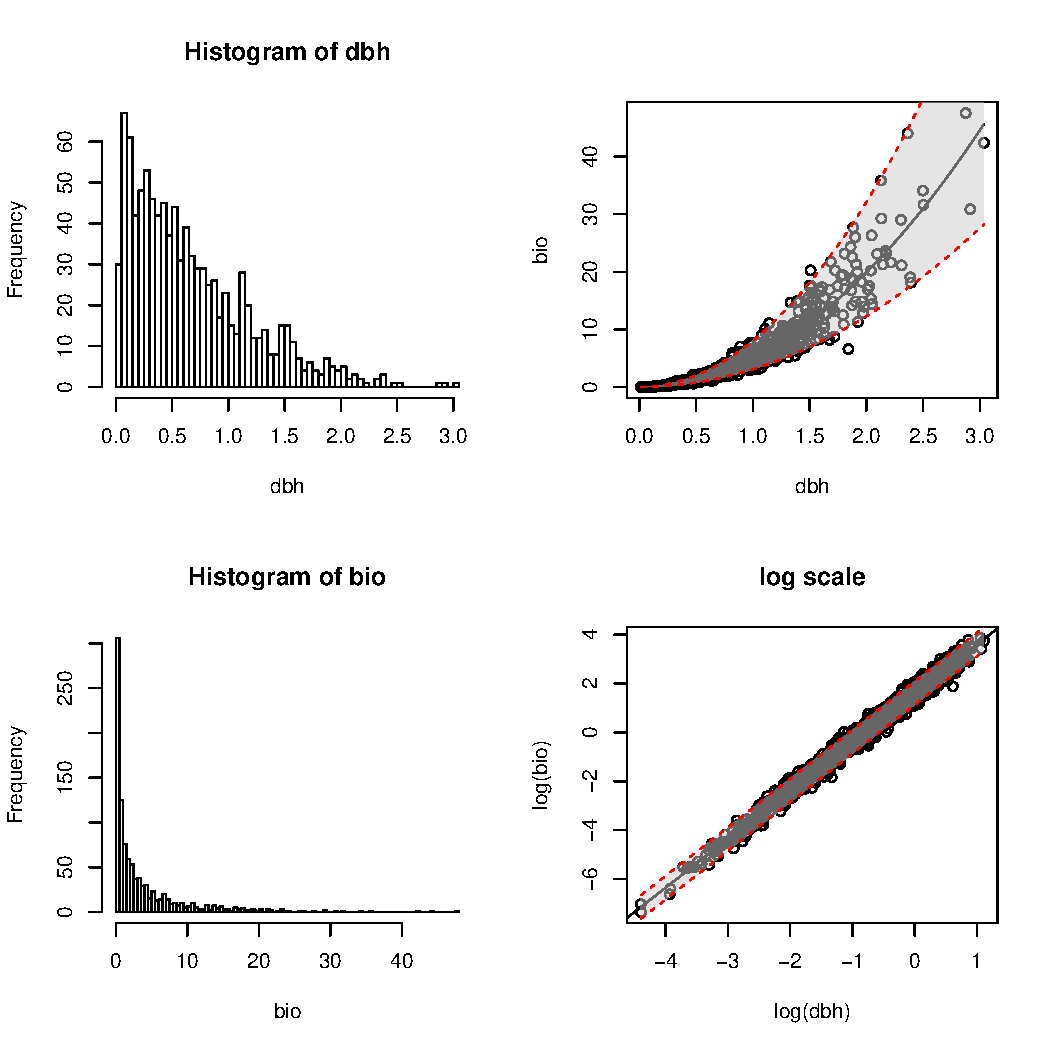
\includegraphics[scale = 0.25]{dbhModel}
  \end{figure}
\end{frame}
%
\begin{frame}
  \frametitle{The Model}
The allometric model is estimated by using ordinary least squares on the log-log model\\
  \begin{align}
  \label{2}
    \log(y_i) & = \beta_0 + \beta_1 \log(x_i) + \epsilon
  \end{align}
  \begin{figure}
    \centering
    \caption{Plot of simulated log-allometric relationship typical of a sample plot (assumes one species only)}
    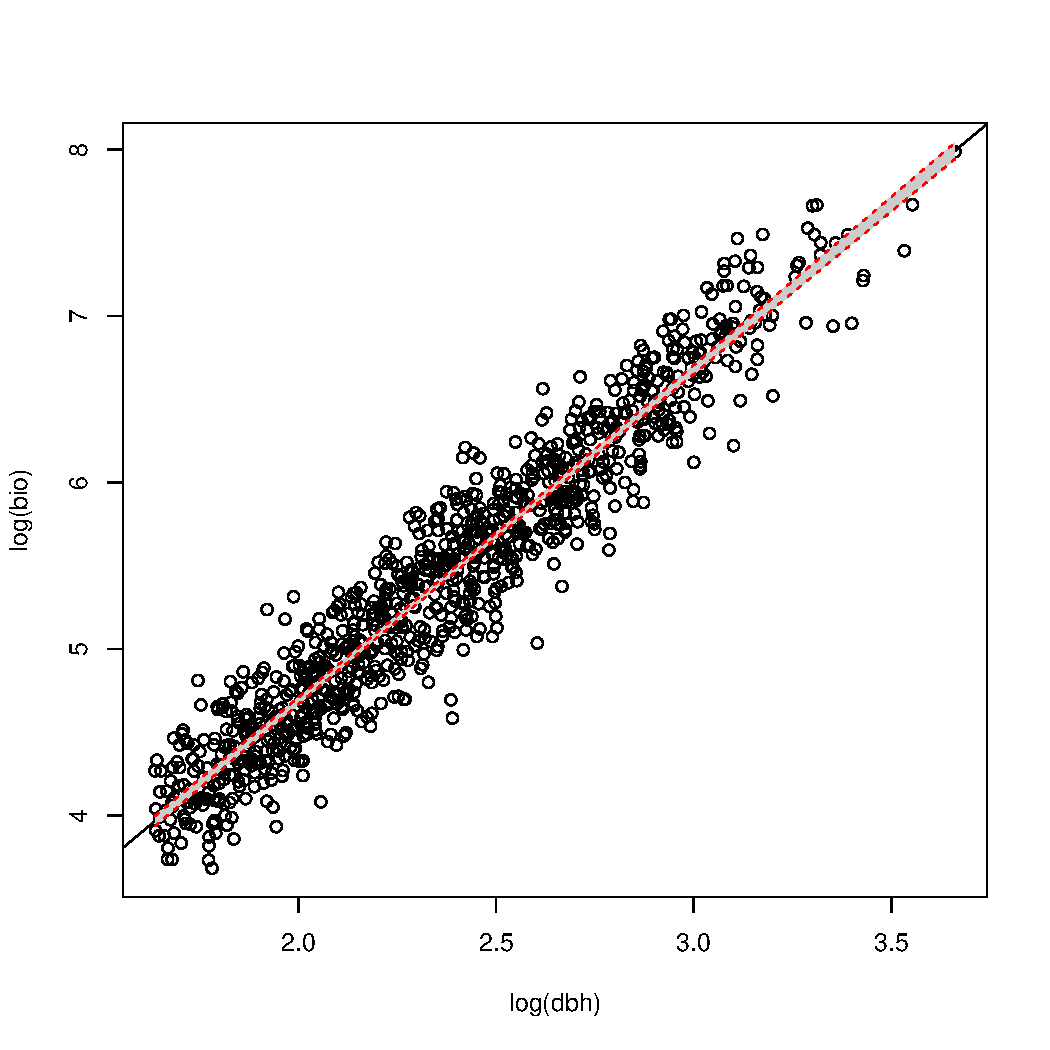
\includegraphics[scale = 0.15]{dbhLogModel}
  \end{figure}
\end{frame}
%
\begin{frame}
  \frametitle{Questions of Interest}
%   Three questions:
  Main questions:
  \begin{enumerate}
  \item What is the effect of sampling design on the estimate of total biomass and its variance estimator \vspace{3mm}
%   \item What is the effect of sampling design on the estimation of the coefficients $\beta_0$ and $\beta_1$ and the estimation of the variances associated with the coefficients $\beta_0$ and $\beta_1$ \vspace{3mm}
  \item How to optimize the sampling design for the desired sampling goals of estimating the total plot biomass with high precision while selecting large trees
  \end{enumerate}
\end{frame}
%
\begin{frame}
  \frametitle{Horvitz-Thompson Estimation}
  \section{Horvitz-Thompson Estimation}
  For a finite population with elements indexed by $i = 1, \ldots, N$ with a probability $\pi_i$ of being included in the sample $s$, the unbiased estimate of the population total is 
  \begin{align*}
    \hat{t}_\pi &  = \sum_{k \in s} \frac{y_k} {\pi_k}.
  \end{align*}
  where $y_i$ is the biomass(or other variable of interest) for tree $i$.\vspace{3mm}
  Estimation of the variance of the population total is calculated as
  \begin{align*}
    \hat{V}(\hat{t}_\pi) &  = \sum_{k \in s} \sum_{l \in s} \frac{1} {\pi_{kl}} \left( \frac{\pi_{kl}} {\pi_k \pi_l} - 1 \right) y_k y_l
  \end{align*}
\end{frame}
%%
%% Add in variance estimator and regression estimator
%%


%
% \section{Finite Population Design}
%   Consider a finite population of size $N$ derived from a continuous distribution. Denote this population $U = \{1, \ldots, N\}$. A simple and easy way to reduce variance in the estimation of a population total is the use of stratified sampling. Stratified sampling is accomplished by sampling from groupings of the ancillary variable $X$ known a priori. For instance, if the values of $X$ are grouped small, medium, and large, a stratified design consists of sampling $n_1$ elements form the small group, $n_2$ elements from the medium group, and $n_3$ elements from the large group. In general, this is extended to $h$ strata where the size of stratum $h$ is known and denoted $N_h$ and the population size is 
%   \begin{align*}
%     N & = \sum_{h = 1}^H N_h. 
%   \end{align*}
% The population total is
%   \begin{align*}
%     t_y & = \sum_{i \in U} y_i\\
%     & = \sum_{h = 1}^H t_h\\
%     & =\sum_{h = 1}^H N_h \bar{y}_h
%   \end{align*}
% where $t_h$ is the stratum total and $\bar{y}_h$ is the stratum mean. In stratified sampling, the $\pi$ estimator for the population total is 
%   \begin{align*}
%     \hat{t}_\pi & = \sum_{h = 1}^H \hat{t}_{h \pi}
%   \end{align*}
% where $\hat{t}_h$ is the $\pi$ estimator of $t_h$. The variance of the estimator $\hat{t}_\pi$ is given by
%   \begin{align*}
%     V(\hat{t}_\pi) & = \sum_{h = 1}^H V(\hat{t}_{h \pi})
%   \end{align*}
% where $V(\hat{t}_{h \pi})$ is the stratum variance of the stratum total $\hat{t}_{h \pi}$. An unbiased variance estimator for the stratified design is 
%   \begin{align*}
%     \hat{V}(\hat{t}_\pi) & = \sum_{h = 1}^H \hat{V}(\hat{t}_{h \pi})
%   \end{align*}
% where $V(\hat{t}_{h \pi})$ is the estimated stratum variance. Within each stratum $h$, a simple random sample of size $n_h$ can be taken. Under this design $s_h$ for sampling stratum $h$, the $\pi$ estimator for the population total $\sum_{i \in U} y_i$ is 
%   \begin{align*}
%     \hat{t}_{\pi} & = \sum_{h = 1}^H N_h \bar{\bm{y}}_{s_h}
%   \end{align*}
% where $\bar{\bm{y}}_{s_h} = \sum_{i \in s_h} \frac{y_i} {n_h}$ is the sample mean for stratum $h$. The variance for the estimator of the population total is 
%   \begin{align*}
%     V(\hat{t}_\pi) & = \sum_{h = 1}^H N_h^2 \frac{1 - f_h} {n_h} s^2_{y U_h}
%   \end{align*}
% where $f_h = \frac{n_h} {N_h}$ is the sampling fraction in stratum $h$ and 
%   \begin{align*}
%     s^2_{y U_h} = \frac{1} {N_h - 1} \sum_{i \in U_h} (y_i - \bar{y}_{U_h})^2    
%   \end{align*}
% is the stratum variance and $\bar{y}_{U_h} = \sum{i \in U_h} \frac{y_i} {N_h}$ is the stratum mean. An unbiased estimator of the variance is 
%   \begin{align*}
%     \hat{V}(\hat{t}_\pi) & = \sum_{h = 1}^H N_h^2 \frac{1 - f_h} {n_h} s^2_{y s_h}
%   \end{align*}
% where
%   \begin{align*}
%     s^2_{y s_h} = \frac{1} {n_h - 1} \sum_{i \in s_h} (y_i - \bar{y}_{s_h})^2
%   \end{align*}
% is the stratum variance in stratum $h$. The mean plot biomass can then be calcualted as $\frac{\hat{t}_\pi} {N}$ and the variance estimator for the mean plot biomass is $\frac{1} {N^2} \hat{V}(\hat{t}_\pi)$.
% 
%

%
\begin{frame}
  \begin{itemize}
    \item The log model can be estimated by using weighted least squares regression with the weight matrix $W = diag(\pi_1, \ldots, \pi_N)$ \vspace{3mm}
    \item Weighted least squares regression model estimate for $\beta$ is $\hat{\beta} = (X^T W X)^{ - 1} X^T W y$ \vspace{3mm}
  \end{itemize}
\end{frame}
%
\begin{frame}
  \section{Sampling Designs}
%
  Five different sampling schemes were considered %% Others to consider are Bitterlich sampling (similar to PPS, selection probability depends on tree size and distance from plot center) - definitely worth pursuing - See Gregorie and Valentine
  %% Stacked radius plots would be similar to STSI 
  %% Can work on including these, but it would require re-writing the simulation code to include locations
  \begin{enumerate}
    \item Simple random sampling (SRS)
    \item Empirical cumulative distribution function (ECDF)
    \item Probability proportional to size sampling (PPS)
    \item Adaptive estimation of the ECDF (AECDF)
%     \item Adaptive estimation of the PPS design (APPS)
    \item Stratified sampling with simple random sampling within each stratum (STSI)
  \end{enumerate}
\end{frame}
%
\begin{frame}
  \frametitle{Simple random sampling (SRS)}
  \begin{itemize}
    \item Easy to implement in the field  \vspace{3mm}
    \item Fails to preferentially select large dbh trees \vspace{3mm}
    \item Baseline for comparison of precision \vspace{3mm}
    \item Example sampling protocol:\vspace{3mm}
    \begin{itemize}
      \item Count the number $N$ of trees at the plot and sample $n$ without replacement
    \end{itemize}    
  \end{itemize}
\end{frame}
%
\begin{frame}
  \frametitle{Probability Proportional to Size (PPS)}
  \begin{itemize}
    \item PPS sampling assigns sample inclusion probabilities based on a size variable known for all elements in the sample, in our case dbh \vspace{3mm}
    \item PPS sampling assigns sample weights for element $i$ of $\pi_i = \frac{dbh_i} {\sum_{i \in U} dbh_i}$ \vspace{3mm}
    \item Highly efficient. This scheme will increase precision more than any other method \vspace{3mm}
    \item PPS sampling will preferentially sample larger dbh trees \vspace{3mm}
    \item Example sampling procedure \vspace{3mm}
    \begin{itemize}
      \item Measure dbh and label all trees in the plot to allow re-visit. Decide which tree to core using a tablet or cellphone with probability of being sampled proportional to size.
    \end{itemize}
  \end{itemize}
\end{frame}
%
\begin{frame}
  \frametitle{Empirical Cumulative Distribution Function Sampling ECDF}
  \begin{itemize} 
    \item ECDF sampling assigns sample inclusion probabilities based on the finite population empirical distribution function $F(\cdot)$ where $F(x_{(n)}) = \frac{n} {N}$ for $x_{(n)}$ the $n^{th}$ order statistic \vspace{3mm}
%    \item This requires knowing the values of the dbh a priori \vspace{3mm}
    \item ECDF provides a point of comparison of the AECDF method as the ECDF is a best case scenario of the AECDF method \vspace{3mm}
    \item ECDF will preferentially sample larger trees \vspace{3mm}
    \item Example sampling procedure: \vspace{3mm}
    \begin{itemize}
      \item  Measure dbh and label all trees in the plot to allow re-visit. Decide which tree to core using a tablet or cellphone with probability of being sampled proportional to the ECDF of dbh.
    \end{itemize}
  \end{itemize}    
\end{frame}
%
\begin{frame}
  \frametitle{Stratified Sampling (STSI)}
  \begin{itemize}
%    \item STSI sampling assigns sample inclusion probabilities for different size classes according to a simple random sampling scheme \vspace{3mm}
    \item STSI groups similar elements of the population and thus increases the precision of estimates by reducing within group variances \vspace{3mm}
    \item STSI sampling can be made to preferentially sample larger trees \vspace{3mm}
    \item Example sampling procedure: \vspace{3mm}
    \begin{itemize}
      \item Decide on a criteria for separating trees into class sizes $h = 1, \ldots H$ (e.g. small, medium, large). At the plot estimate the number of trees in each class size $N_h$ (this does not have to be exact, just close). Using a cellphone/tablet, randomly sample $n_h$ trees from each class $h$. 
    \end{itemize}
  \end{itemize}
\end{frame} 
%
\begin{frame}
  \frametitle{Adaptive ECDF sampling (AECDF)}
  \begin{itemize}
    \item AECDF asymptotically approaches the ECDF design \vspace{3mm}
    \item AECDF preferentially samples larger dbh trees \vspace{3mm}
    \item AECDF variance estimator will need to be derived mathematically (not currently solved to the best of my knowledge) \vspace{3mm}
    \item Example sampling procedure: \vspace{3mm}
    \begin{itemize}
      \item Measure the dbh of the first tree at the plot. Sample a tree core for this first tree. At the second tree, measure dbh and sample according to up-down decision using smartphone or computer. Continue through the plot in this fashion. This design produces a random (but controllable) sample size.
    \end{itemize}
  \end{itemize}
\end{frame}
%
% \begin{frame}
%   \frametitle{Adaptive PPS sampling (APPS)}
%   \begin{itemize}
%     \item APPS asymptotically approaches the PPS design \vspace{3mm}
%     \item APPS preferentially samples larger dbh trees \vspace{3mm}
%     \item APPS variance estimator will need to be derived mathematically (not currently solved to the best of my knowledge) \vspace{3mm}
%     \item Example sampling procedure:
%     \begin{itemize}
%       \item Measure the dbh of the first tree at the plot. Sample a tree core for this first tree. At the second tree, measure dbh and sample according to up-down decision using smartphone or computer. Continue through the plot in this fashion. This design produces a random (but controllable) sample size.
%     \end{itemize}
%   \end{itemize}
% \end{frame}
%
\begin{frame}
  \section{Simulation and results}
  Using the simulated data presented earlier, I repeatedly sampled $n = 10, 40,$ and $100$ trees from the simulated population of $N = 400$ trees using the proposed designs and calculated Monte Carlo bias and relative efficiencies for each design based on 10,000 replicates. 
\end{frame}
%
\begin{frame}
  \frametitle{Results $n = 20$}
  % latex table generated in R 3.0.2 by xtable 1.7-1 package
  % Wed Feb  5 15:13:08 2014
  \begin{table}[ht]
  \centering
  \begin{tabular}{rrr}
    \hline
    & Bias & Relative Efficiency \\ 
    \hline
    SRS & -0.00 & 1.00 \\ 
    ECDF & -0.01 & 0.71 \\ 
    PPS & -0.04 & 0.13 \\ 
    AECDF & 0.06 & 1.40 \\ 
%     APPS & -0.02 & 0.47 \\ 
    STSI & 0.00 & 0.48 \\ 
   \hline
  \end{tabular}
  \end{table}
\end{frame}
%
\begin{frame}
  \frametitle{Results $n = 40$}
  % latex table generated in R 3.0.2 by xtable 1.7-1 package
  % Wed Feb  5 15:01:30 2014
  \begin{table}[ht]
  \centering
  \begin{tabular}{rrr}
    \hline
    & Bias & Relative Efficiency \\ 
    \hline
    SRS & -0.02 & 1.00 \\ 
    ECDF & -0.00 & 0.73 \\ 
    PPS & -0.07 & 0.14 \\ 
    AECDF & 0.01 & 1.41 \\ 
%     APPS & 0.00 & 0.36 \\ 
    STSI & -0.00 & 0.37 \\ 
     \hline
  \end{tabular}
  \end{table} 
\end{frame}
%
\begin{frame}
  \frametitle{Results $n = 100$}
  % latex table generated in R 3.0.2 by xtable 1.7-1 package
  % Wed Feb  5 15:18:44 2014
  \begin{table}[ht]
  \centering
  \begin{tabular}{rrr}
    \hline
    & Bias & Relative Efficiency \\ 
   \hline
    SRS & 0.01 & 1.00 \\ 
    ECDF & 0.00 & 0.54 \\ 
    PPS & -0.27 & 0.10 \\ 
    AECDF & 0.04 & 1.45 \\ 
%     APPS & -0.00 & 0.56 \\ 
    STSI & 0.00 & 0.55 \\ 
   \hline
  \end{tabular}
  \end{table}
\end{frame}
%
\begin{frame}
  \frametitle{Results for sampling for biomass}
  \section{Results}
  \begin{enumerate}
    \item Relative efficiency is a measure of the expected decrease in variance for a given sample size and design relative to SRS. A relative efficiency of 0.25 implies the design of interest has 1/4 of the variance of SRS design (equivalently the design requires $\sqrt{1/4} = 1/2$ the sample size to achieve the same efficiency).
    \item Two designs perform well in the simulation, PPS, and STSI. Of these designs, STSI is the easiest to implement in field while PPS is more powerful. STSI can be tuned to sample the distribution of dbh (and hence biomass and age)
    \item Fixed radius nested plot sampling is similar to STSI sampling and Bitterlich sampling is similar to PPS sampling.
%     \item Note that this simulation also includes uncertainty in estimating the allometric model coefficients $\hat{\beta}$ and using known values would increase efficiency further
  \end{enumerate}
\end{frame}
%
\begin{frame}
  \frametitle{Sampling for age (longer chronologies)}
  \begin{itemize}
    \item The results for sampling older trees should be comparable to these designs sampling biomass, as long as the correlation between age and dbh is similar to the correlation between biomass and dbh. As this level of correlation decreases, the efficiency gains due to STSI and PPS sampling decrease as well
    \item Currently we are investigating a sub-sampling scheme using real data to show similar results for tree age as we have for biomass.
  \end{itemize}
\end{frame}
%
% \begin{frame}
%   \section{Appendix - Current discussion items, thoughts, hypotheses, and other trains of thought}
%   \begin{itemize}
%     \item First, we need to pin down the primary questions of interest and define the goals
%     \begin{itemize}
%       \item Is the goal to sample large trees that will likely have a longer chronology and thus allow a better back forecast of biomass in a probabilistic way?
%       \item Is the goal to decrease the uncertainty about biomass for large values of dbh?
%       \item Is the goal to develop an adaptive sampling design that can be implemented in field to preferentially select larger trees in a statistically sound way while maintaining a probabilistic sample or is it to design a robust sampling design that is easy to implement?
%     \end{itemize}
%     \item Does the design need to incorporate multiple species? perhaps you could stratify based on size and species?
%   \end{itemize}
% \end{frame}
%
\end{document}
